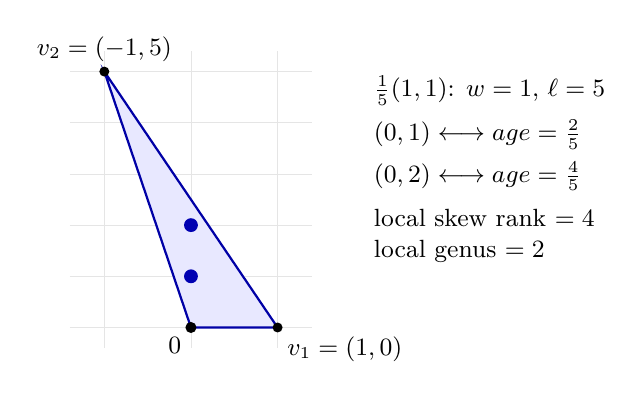
\begin{tikzpicture}[x=1.1cm,y=0.65cm,font=\small]
  \draw[step=1,gray!20,very thin] (-1.4,-0.4) grid (1.4,5.4);
  \filldraw[fill=blue!9,draw=blue!65!black,thick] (0,0)--(1,0)--(-1,5)--cycle;
  \fill (0,0) circle (2pt) node[below left] {$0$};
  \fill (1,0) circle (1.8pt) node[below right] {$v_1=(1,0)$};
  \fill (-1,5) circle (1.8pt) node[above] {$v_2=(-1,5)$};
  \fill[blue!70!black] (0,1) circle (2.5pt);
  \fill[blue!70!black] (0,2) circle (2.5pt);
  \node[anchor=west,align=left] at (2,3.1)
    {$\frac15(1,1)$: $w=1$, $\ell=5$\\[5pt]
     $(0,1)\longleftrightarrow\operatorname{age}=\frac25$\\[4pt]
     $(0,2)\longleftrightarrow\operatorname{age}=\frac45$\\[5pt]
     local skew rank $=4$\\
     local genus $=2$};
\end{tikzpicture}